\chapter{Clustering}

In the field of clustering analysis, there is no strict definition for cluster itself. That may be one reason why there is such a vast amount of clustering algorithms; many papers such as \cite{estivill2002so} address this topic.  However, the one think in common that we can find among all the algorithms is a work with a group of data objects.

Suppose data $\mathcal{D}$ given as a $n$ $d$-dimensional vectors $(x_1,\dots,x_d) \subset \R_d$  -- objects; each element of a vector describes specific object property. Two objects are similar if values of their respective properties are alike. Then, clustering analysis can be defined as a form of grouping objects into subsets of $\mathbf{D}$ while maximizing inter-set object similarity and minimizing intra-set object similarity.

\section{Clustering models}

Concrete variations of clustering analysis are defined by a clustering model. They are divided into several sections.

\subsection{Centroid-based model}

\emph{Centroid-based clustering model} represents clusters only by a central vector --- \emph{centroid} --- which is not necessarily a member of a working set. Many implementations of this model need the number of required centroids in advance. We define the following optimalization problem for this kinds of algorithms. 

\begin{problem}
	Having a distance function $d$, find $k$ centroids $C_1,\dots,C_k$ from the domain of the dataset $\mathcal{D}$ such that the sum \ref{eq01:sum}
	is minimized.
\end{problem}

\begin{equation}\label{eq01:sum}
	\sum_o^{\mathcal{D}} \min_{i=1\dots k}d(o,C_i)
\end{equation}

This problem is uneasy to solve due to its exponential complexity. Hence, many approximation algorithms emerged. 

\subsubsection{k-means}

The most common implementation of centroid-based clustering is \emph{k-means}. Its algorithm can be expressed in a few simple steps:

\begin{Verbatim}[commandchars=\\\{\},codes={\catcode`$=3\catcode`^=7\catcode`_=8},frame=lines,label=$k$-means]
[0]  initialize dataset $\mathcal{D}$
[1]  choose first $k$ objects from $\mathcal{D}$ as centroids $c_1,\dots,c_k$ 
[2]  $\mathcal{C}$ <- $\{c_1,\dots,c_k\}$
[3]  do
[4]    for each $c_i$ create empty cluster $K_i$
[5]    for each $o \in \mathcal{D}$ find closest centroid $c_i$; do
[6]      $K_i$ <- $K_i \cup o$
[7]    for each $K_i$ compute new centroid $c^\prime_i$
[8]    $\mathcal{C}^\prime$ <- $\{c^\prime_1,\dots,c^\prime_k\}$
[9]    swap $\mathcal{C}$ and $\mathcal{C}^\prime$
[10] while $\mathcal{C}$ != $\mathcal{C}^\prime$
\end{Verbatim}

The algorithm divides data into $k$ clusters (hence, \emph{k}-means) in a iterative manner. Before the first iteration, initial $k$ central vectors are selected from the dataset. Each iteration, dataset objects are grouped into clusters according to the closest centroid. After that, new centroids are then computed from new clusters. Next iteration follows until centroids does not change or predefined number of iterations is reached. 

The advantage of this algorithm is the fact that it is easily comprehensible; hence can sustain for large variety of datasets. Another think is that it is said to be the speediest centroid-based algorithm. However, the disadvantages are inability to deal with the noise in a dataset and clusters of non-convex shape (\cite{uppada2014centroid}).
  

\subsection{Hierarchical model}

In \emph{Hierarchical clustering model}, objects are \emph{connected} together forming tree-like structure. In contrast with the aim of centroid-based model returning only $k$ centroids, hierarchical clustering algorithms capture whole connecting process. The algorithm starts with all objects from a dataset being initial clusters. Each iteration, two clusters are connected creating a new one finishing with one all-inclusive cluster. Commonly, this algorithms represent the connecting process as an ordered list of pairs --- connected clusters (\cite{karypis1999chameleon}).

The above described approach of a hierarchical algorith is called \emph{agglomerative} approach. The algorithm begins with each object representing a cluster on its own. Then, in a bottom-up fashion clusters are successively connected into the only cluster. The other option is \emph{divisive approach}. Beginning with a single all-inclusive cluster it is divided into sub-clusters until single objects remain (\cite{rokach2005clustering}). 

The result of hierarchical clustering can be viewed in a \emph{dendrogram} see \ref{fig01:dendro}. The x-axis states the distance of connected clusters. The y-axix shows the objects from a dataset.

This model distinguishes various kind of hierarical clustering algorithms based on the choice of a \emph{distance function} and so called \emph{linkage criterion}. 

\begin{figure}\centering
	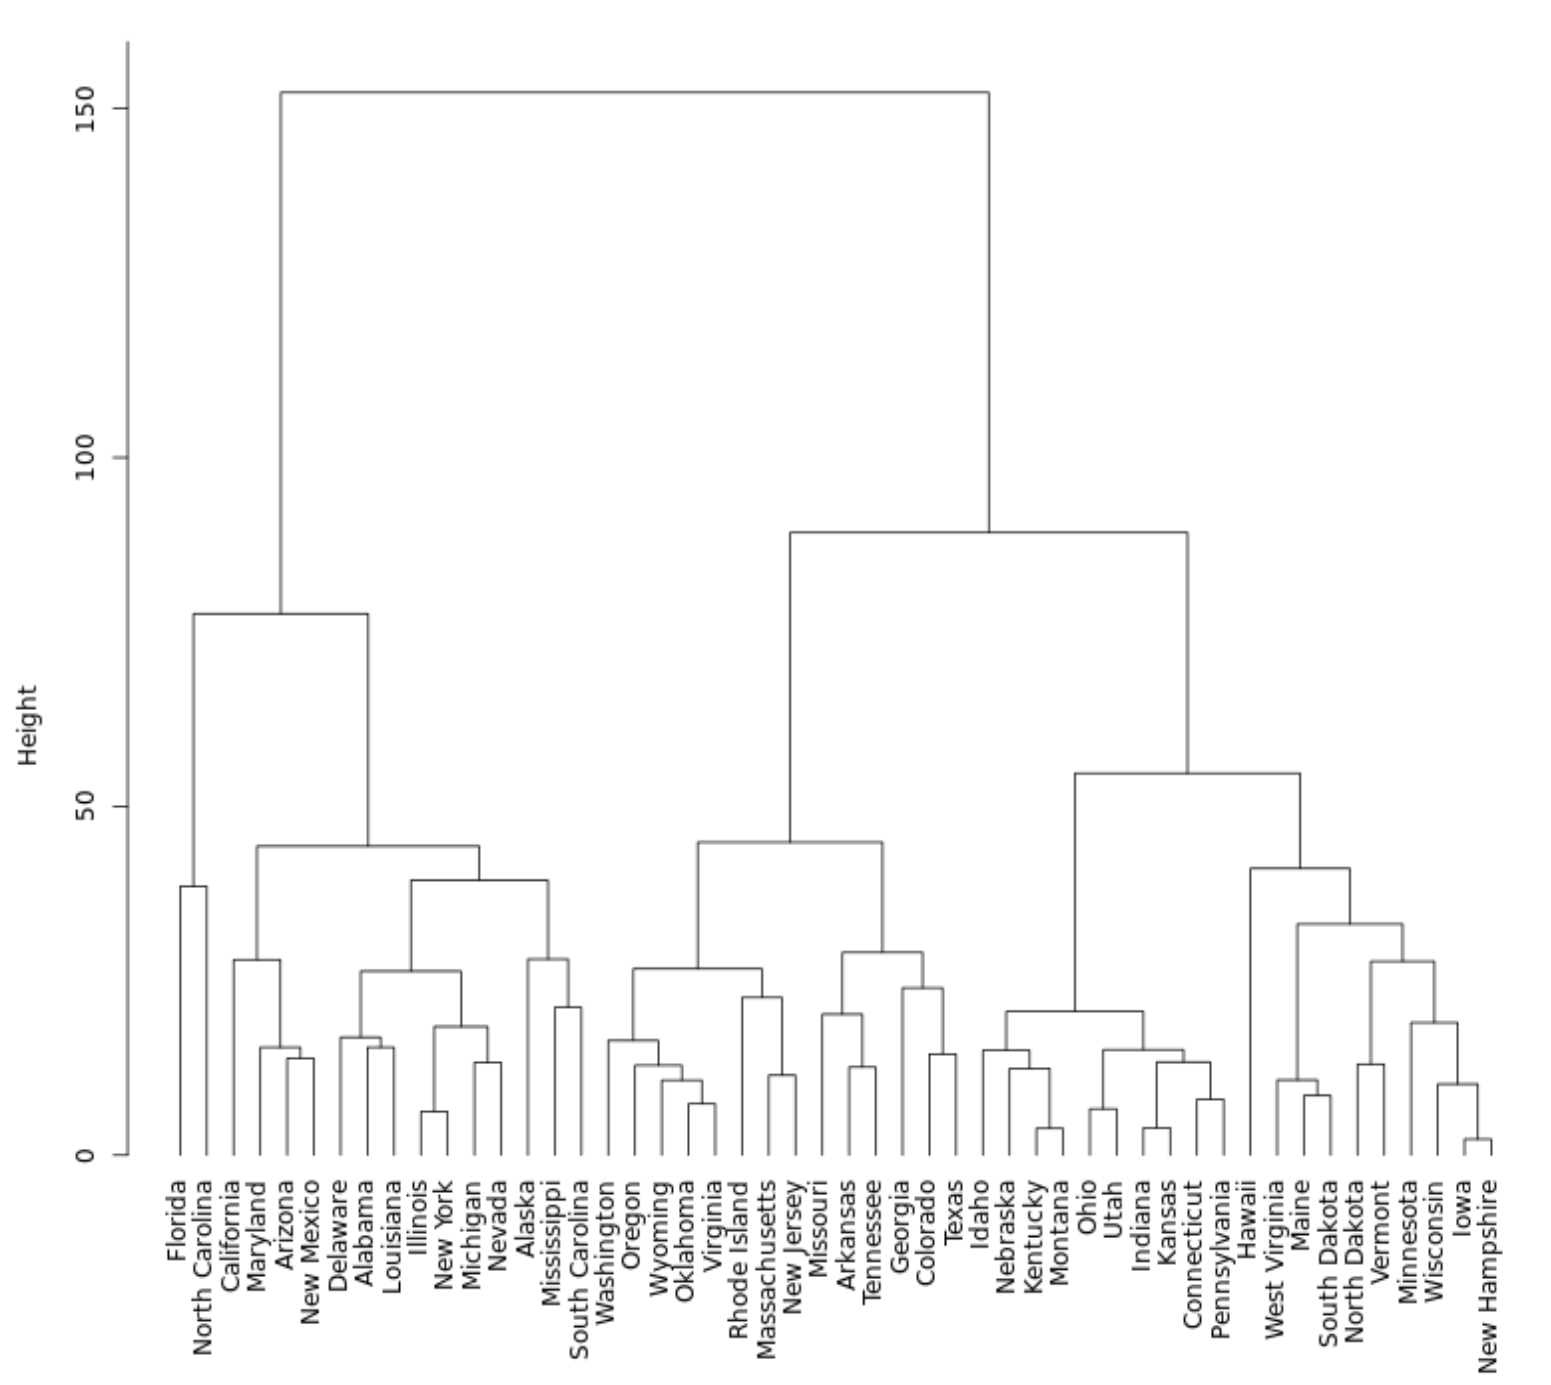
\includegraphics{img/dendro}
	\caption{An example of dendrogram.}
	\label{fig01:dendro}
	
\end{figure}

\subsection{some hierarchical clusterings}

examples

\subsection{mahalanobis clustering}

definition, variations

\subsection{performance}

comparison